\documentclass{beamer}

\mode<presentation>

\title{Symbolic Music Similarity}
\subtitle{Presentation}
\author{Ali Bektas \and Paul Kröger}

\usepackage{graphicx}
\graphicspath{{./images/}}
\usepackage{verbatim}

\begin{document}
	\begin{frame}
		\maketitle
	\end{frame}
	
	\begin{frame}
  		\frametitle{Darstellung von Noten}
  		\begin{minipage}{0.45\textwidth}
  			\begin{itemize}
			\item Melodie : \textit{"singbare, in sich geschlossene Folge von Tönen"} \cite{duden_melodie}
			\item Harmonie : \textit{"wohltönender Zusammenklang mehrerer Töne oder Akkorde"} \cite{duden_harmonie}
			\item Schlüssel : \textit{"dient in der Musiknotation dazu, im Notensystem festzulegen, welche Tonhöhe die fünf Notenlinien repräsentieren."} \cite{def_schlussel}
			\end{itemize}
		\end{minipage}%
		\begin{minipage}{0.45\textwidth}
			\begin{figure}[h!]
				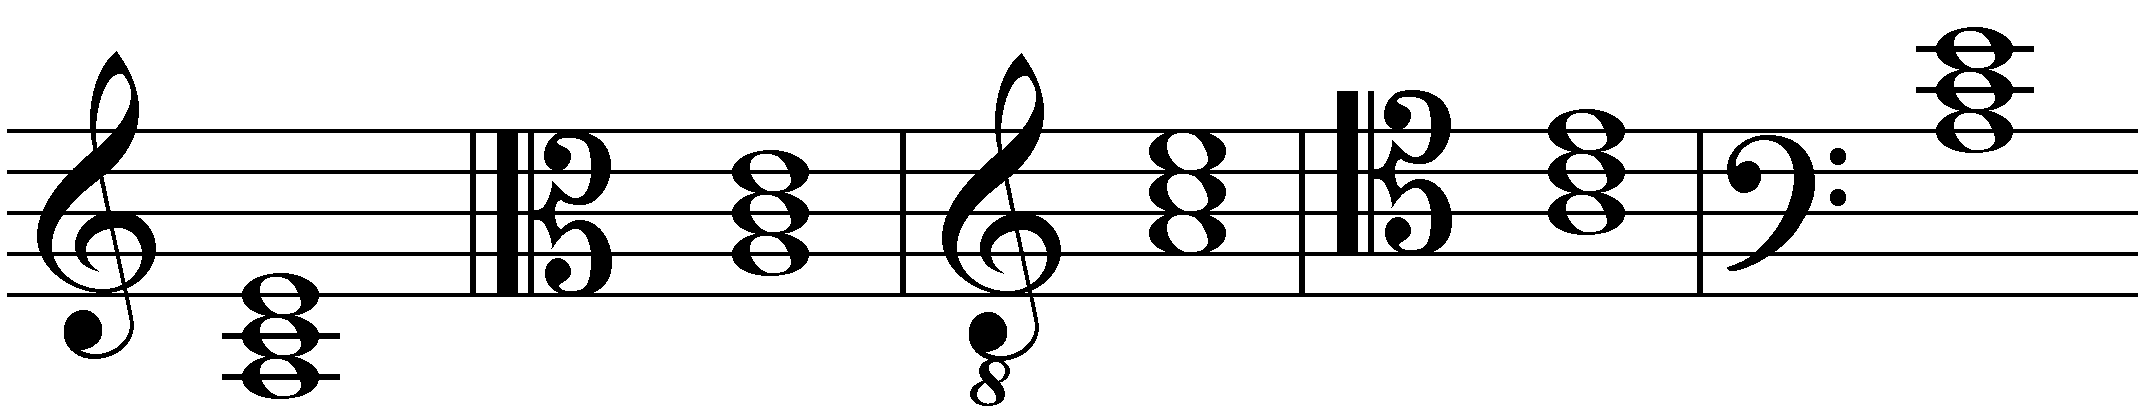
\includegraphics[width=100px,height=100px,keepaspectratio]{Clefs_chord}
				\caption{Source: \cite{def_schlussel}}
			\end{figure}
		\end{minipage}
	\end{frame}

	\begin{frame}
		\frametitle{Darstellung von Noten}
		Im Grunde genommen , ermöglicht die herkömmliche Methode von Notendarstellung , Informationen über Rhytmus , Tonlage , Gefühl beim Spielen , vortragsbetreffliche Elemente zu übermitteln.
		\begin{figure}[h!]
			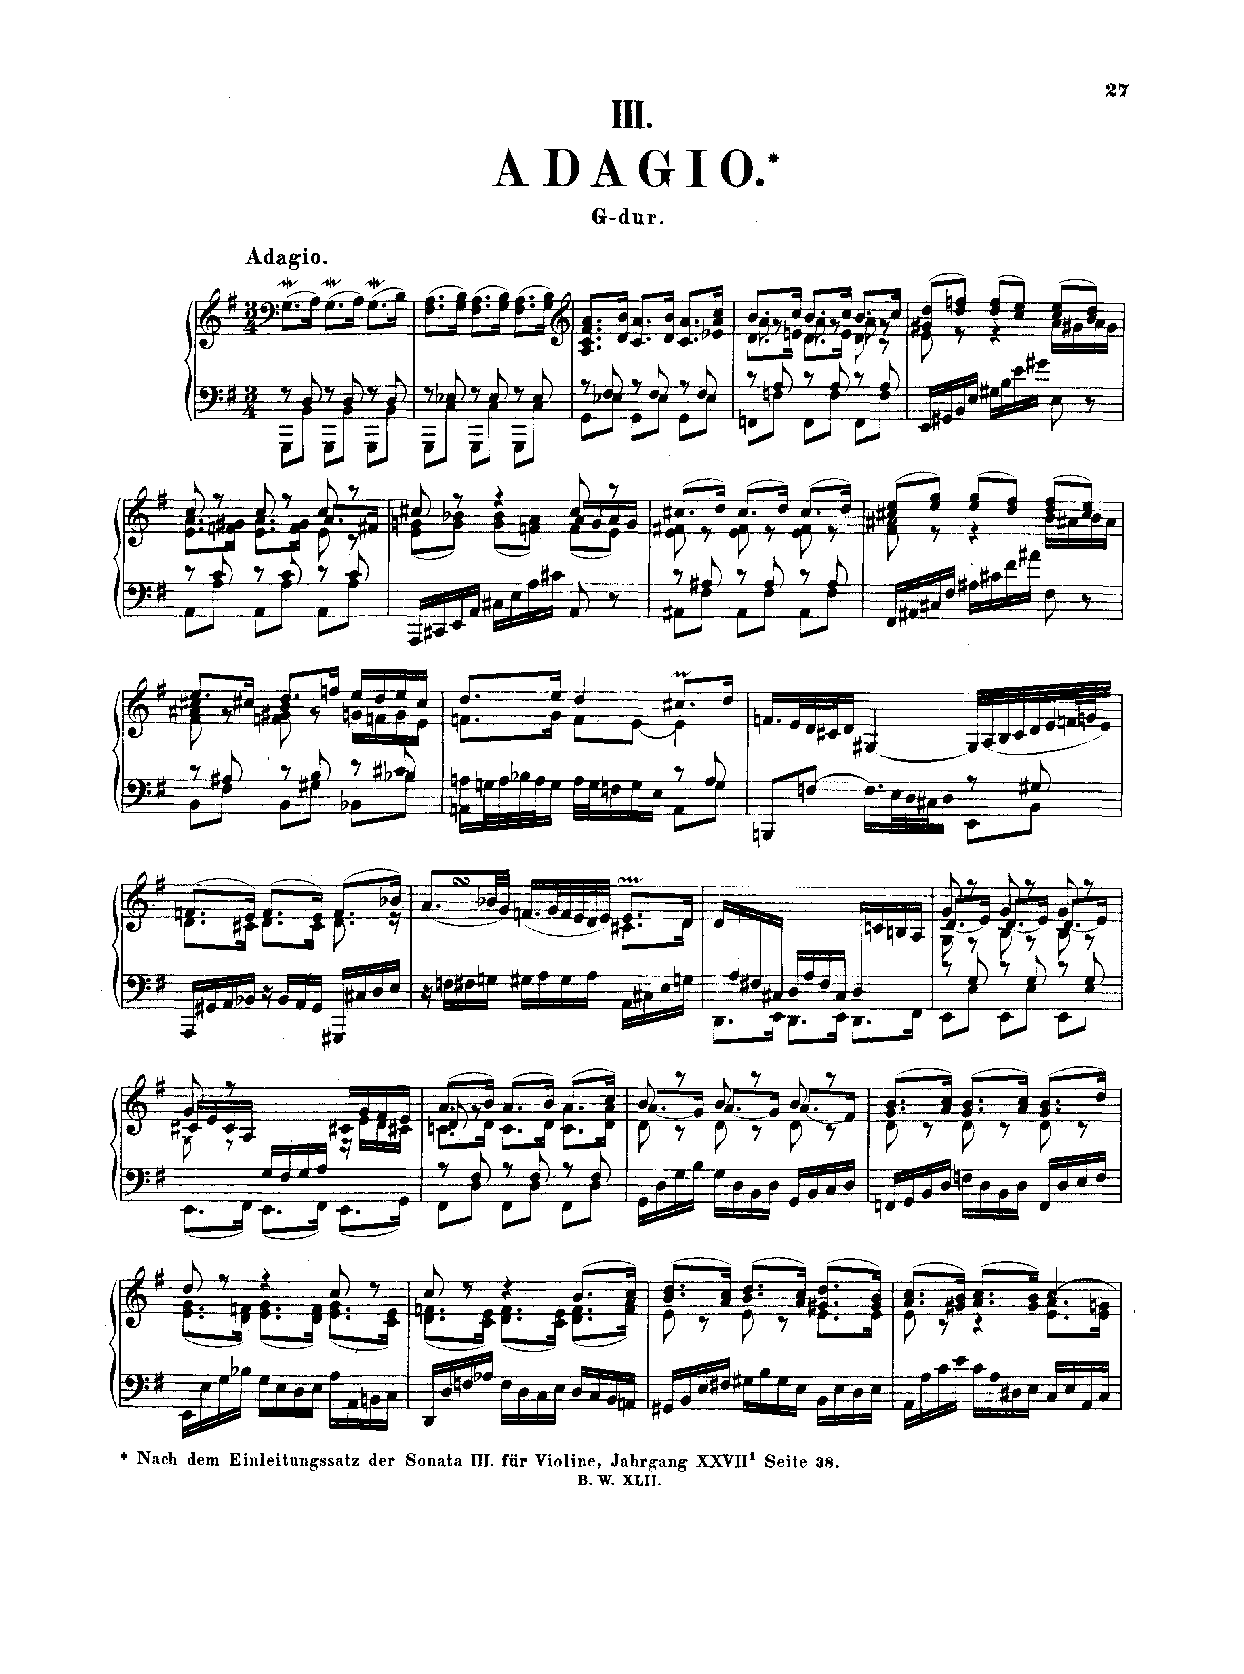
\includegraphics[width=300px,height=150px,keepaspectratio]{bach_adagio}
			\caption{Source: IMLSP Archive}
		\end{figure}
	\end{frame}

	\begin{frame}
		\frametitle{MIREX}
		\begin{itemize}
			\item Ein Wettbewerb und Plattform für Interessierte
			\item Es gibt verschiedene Kategorien
				\begin{itemize}
					\item Real-time Audio to Score Alignment (a.k.a Score Following)
					\item Discovery of Repeated Themes and Sections
					\item Audio Melody Extraction
					\item \textbf{Symbolic Melodic Similarity}
					\item ...
				\end{itemize}
			\item Gegeben ein Ziel , treten verschiedene Algorithmen gegeneinander zum Wettkampf an. Derjenige, der die besten Ergebnisse hat , gewinnt. 
			\item \textbf{Nun eine Frage:}Wie kann man Algorithmen miteinander vergleichen?
			\item Es kommt nicht auf die Laufzeit oder Speicherbedarf an , sondern auf die Qualität der Ergebnisse.
			\item Welche Messmethoden gibt es , um die Qualität von solcen Ergebnissen zu beurteilen?
		\end{itemize}
	\end{frame}

	\begin{frame}
		\frametitle{MIREX}
		\begin{figure}[h!]
			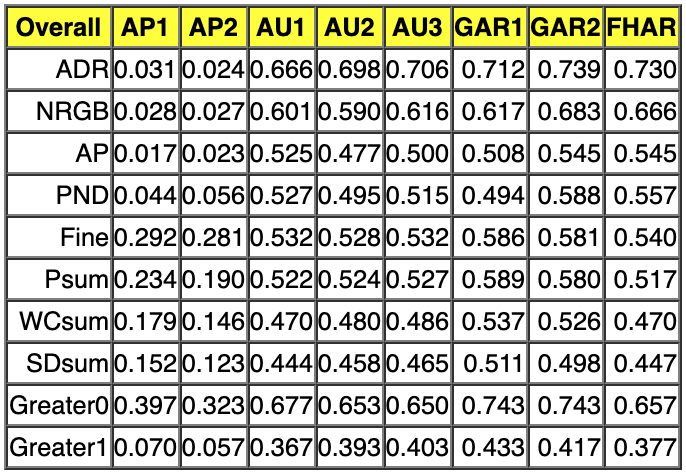
\includegraphics[width=300px,height=150px,keepaspectratio]{mirex_result_example}
			\caption{Source: \cite{mirex_website_2007_results}}
		\end{figure}
	\end{frame}


	\begin{frame}
		\frametitle{MIREX}
		\begin{figure}[h!]
			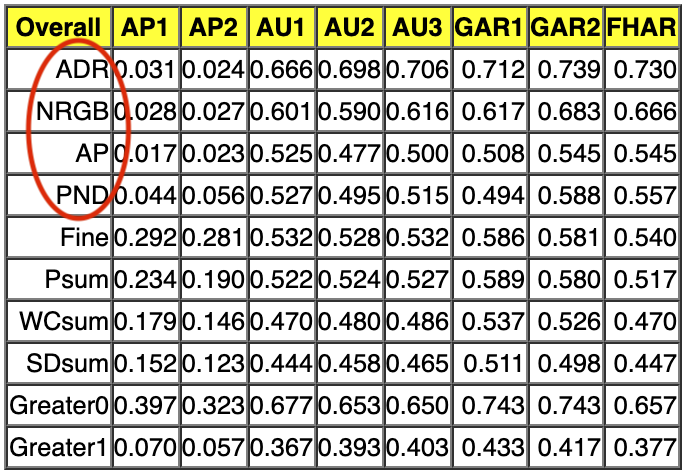
\includegraphics[width=300px,height=150px,keepaspectratio]{mirex_result_example_change_one}
		\end{figure}
	\end{frame}

	\begin{frame}
		\frametitle{Average Dynamic Recall - ADR}
		
	\end{frame}

	\begin{frame}
		\frametitle{MIREX}
		\begin{figure}[h!]
			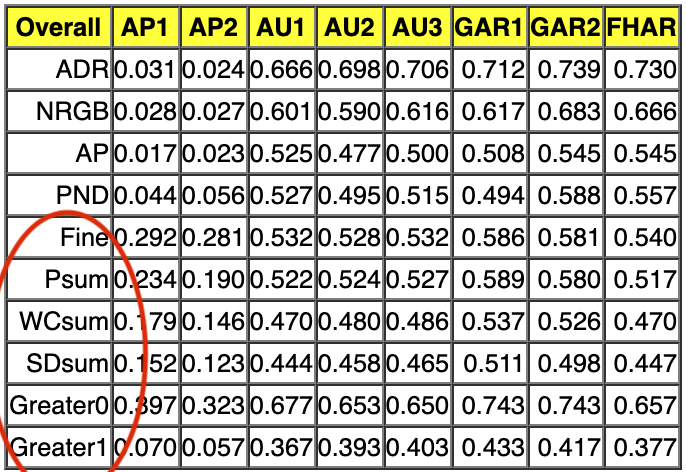
\includegraphics[width=300px,height=150px,keepaspectratio]{mirex_result_example_change_two}
		\end{figure}
	\end{frame}

	\begin{frame}
		\frametitle{Bibliographie}
		\begin{thebibliography}{5}
			\setbeamertemplate{bibliography item}[text]
			\bibitem[1]{duden_melodie} Duden: Melodie: Rechtschreibung, Bedeutung, Definition, Herkunft
			https://www.duden.de/rechtschreibung/Melodie.
			\bibitem[2]{duden_harmonie} Duden: Harmonie : Rechtschreibung, Bedeutung, Definition, Herkunft
			https://www.duden.de/rechtschreibung/Harmonie.
			\bibitem[3]{def_schlussel} “Notenschlüssel.” Wikipedia, Wikimedia Foundation, 11 Dec. 2019, de.wikipedia.org/wiki/Notenschlüssel.
			\bibitem[4]{mirex_website} MIREX,Symbolic Melodic Similarity 2005,https://www.music-ir.org/mirex/wiki/2005:Symbolic\_Melodic.
			\bibitem[5]{mirex_website_2007_results} MIREX,Symbolic Melodic Similarity Results 2007, https://www.music-ir.org/mirex/wiki/2007:Symbolic\_Melodic\_Similarity\_Results.
		\end{thebibliography}
	\end{frame}
\end{document}